%! TeX root = master.tex
% !TEX program = lualatex

\lecture{4}{2026-10-01}{Mandatory Access Control: confidentiality and integrity models}{}

\section{From DAC to MAC}

\subsection{Recall: who decides the policy?}

We studied \textbf{Discretionary Access Control (DAC)}, where the \emph{owners} of objects assign the permissions. This lecture covers the other family:

\begin{definition}[Mandatory Access Control]
An access control approach in which \textbf{a central security policy assigns the permissions}. Access to, and operations on, resources are determined by the security policy:
\begin{itemize}
    \item an ``owner'' \textbf{may not exist}, or \textbf{may not have the power} to set permissions against the policy;
    \item the security policy \textbf{must be enforced despite subjects trying to subvert it}.
\end{itemize}
\end{definition}

\begin{remark}
The second point is the crucial difference with DAC. Under DAC, a malicious program running with Alice's privileges can simply copy Alice's secret file into a public file, or \texttt{chmod} it, since Alice is the owner. Under MAC, \emph{neither Alice nor her programs} can make the information flow somewhere the central policy forbids.
\end{remark}

This lecture is theoretical on purpose: the goal is to understand basic concepts and principles of security design that will \textbf{outlast current technology}.

\subsection{Security models}

\begin{definition}[Security model]
A \textbf{design pattern} for a specific security property or set of properties.
\end{definition}

When faced with a standard security problem, \textbf{use a well-known model} rather than inventing your own (the same philosophy as ``do not roll your own crypto''). However, many aspects are \emph{not} covered by the model:
\begin{itemize}
    \item who are the \textbf{subjects}?
    \item what are the \textbf{objects}?
    \item what \textbf{mechanisms} are used to implement it?
\end{itemize}
\textbf{The devil is in the details!} A model only tells you what the rules are; mapping a real system onto the model (and implementing the mapping correctly) is where things go wrong.

This lecture presents three models:
\begin{table}[h]
\centering
\begin{tabular}{@{}lll@{}}
\toprule
\textbf{Model} & \textbf{Protects} & \textbf{Typical setting} \\
\midrule
Bell--La Padula (BLP) & Confidentiality & Military, government \\
BIBA & Integrity & Banking, commerce, OS integrity \\
Chinese Wall (Brewer--Nash) & Conflicts of interest (C \& I) & Financial sector, consulting \\
\bottomrule
\end{tabular}
\caption{The three MAC security models of this chapter.}
\end{table}

\section{Bell--La Padula (BLP): protecting confidentiality}

D.\ Bell and L.\ LaPadula, \emph{Secure computer systems: Unified exposition and Multics interpretation}, MITRE Technical Report ESD-TR-75-306, 1976.

\subsection{Subjects, objects and access rights}

Subjects $S$ and objects $O$ are each associated with a \textbf{level of confidentiality}. Subjects' access rights are defined by four attributes:

\begin{table}[h]
\centering
\begin{tabular}{@{}lp{7.3cm}cc@{}}
\toprule
\textbf{Right} & \textbf{Meaning} & \textbf{Observe?} & \textbf{Alter?} \\
\midrule
\textbf{e}xecute & The subject cannot see or modify the object, but can run it & no & no \\
\textbf{r}ead & The subject can only see the object, but cannot modify it & yes & no \\
\textbf{a}ppend & The subject cannot read the object, but can attach new content to it & no & yes \\
\textbf{w}rite & The subject can see the object, add content and modify existing content & yes & yes \\
\bottomrule
\end{tabular}
\caption{The four BLP access rights.}
\end{table}

These access rights are defined in an \textbf{access control matrix} (as in DAC, see the ds-property below).

\begin{remark}[Observe vs.\ alter]
Keep this classification in mind: \textbf{read} and \textbf{write} both \emph{observe}; \textbf{append} and \textbf{write} both \emph{alter}. Write is therefore constrained by \emph{both} BLP rules, which is why it ends up only allowed at the subject's own level.
\end{remark}

\subsection{Security levels of objects: classification}

\begin{definition}[Security level]
A security level is a pair
\[
\text{Security Level} = (\text{Classification}, \{\text{set of categories}\})
\]
where
\begin{itemize}
    \item the \textbf{classification} is a label from a \textbf{total order} (e.g.\ Unclassified $<$ Confidential $<$ Secret $<$ Top Secret);
    \item the \textbf{categories} (or \emph{compartments}) group objects with a common topic (e.g.\ Nuclear, NATO, Crypto).
\end{itemize}
Each object has a security level: it has a label and belongs to zero, one or more categories.
\end{definition}

Categories implement \textbf{need-to-know}: a general with Top Secret clearance in the category NATO should not see Top Secret Nuclear documents unless he also has the Nuclear category.

\subsection{The dominance relationship}

\begin{definition}[Dominance]
A security level $(l_1, c_1)$ \textbf{dominates} $(l_2, c_2)$, written $(l_1, c_1) \succeq (l_2, c_2)$, if and only if
\[
l_1 \geq l_2 \qquad \text{and} \qquad c_2 \subseteq c_1.
\]
\end{definition}

\textbf{Both} conditions must hold: a higher label is useless if a category is missing.

\begin{example}[Hospital]
Labels: Admin $<$ Nurse $<$ Surgeon $<$ Doctor. Categories: DEMOGRAPHICS, ANALYSIS, RESULTS. Which statements are true?
\begin{enumerate}
    \item $(D, \{\}) \succeq (S, \{\})$: \textbf{true} ($D \geq S$ and $\{\} \subseteq \{\}$).
    \item $(S, \{\}) \succeq (N, \{\text{RESULTS}\})$: \textbf{false} ($S \geq N$, but $\{\text{RESULTS}\} \not\subseteq \{\}$).
    \item $(S, \{\text{DEM}, \text{RES}\}) \succeq (N, \{\text{DEM}\})$: \textbf{true} ($S \geq N$ and $\{\text{DEM}\} \subseteq \{\text{DEM}, \text{RES}\}$).
    \item $(D, \{\text{ANA}, \text{RES}\}) \succeq (S, \{\text{DEM}\})$: \textbf{false} ($D \geq S$, but DEM is missing).
\end{enumerate}
\textbf{Which level dominates them all?} $(\text{Doctor}, \{\text{DEM}, \text{ANA}, \text{RES}\})$: highest label and all categories (the \emph{top}).

\textbf{Which level dominates only itself?} $(\text{Admin}, \{\})$: lowest label and no category (the \emph{bottom}). It is dominated by every level.
\end{example}

\subsubsection{The dominance lattice}

\begin{center}
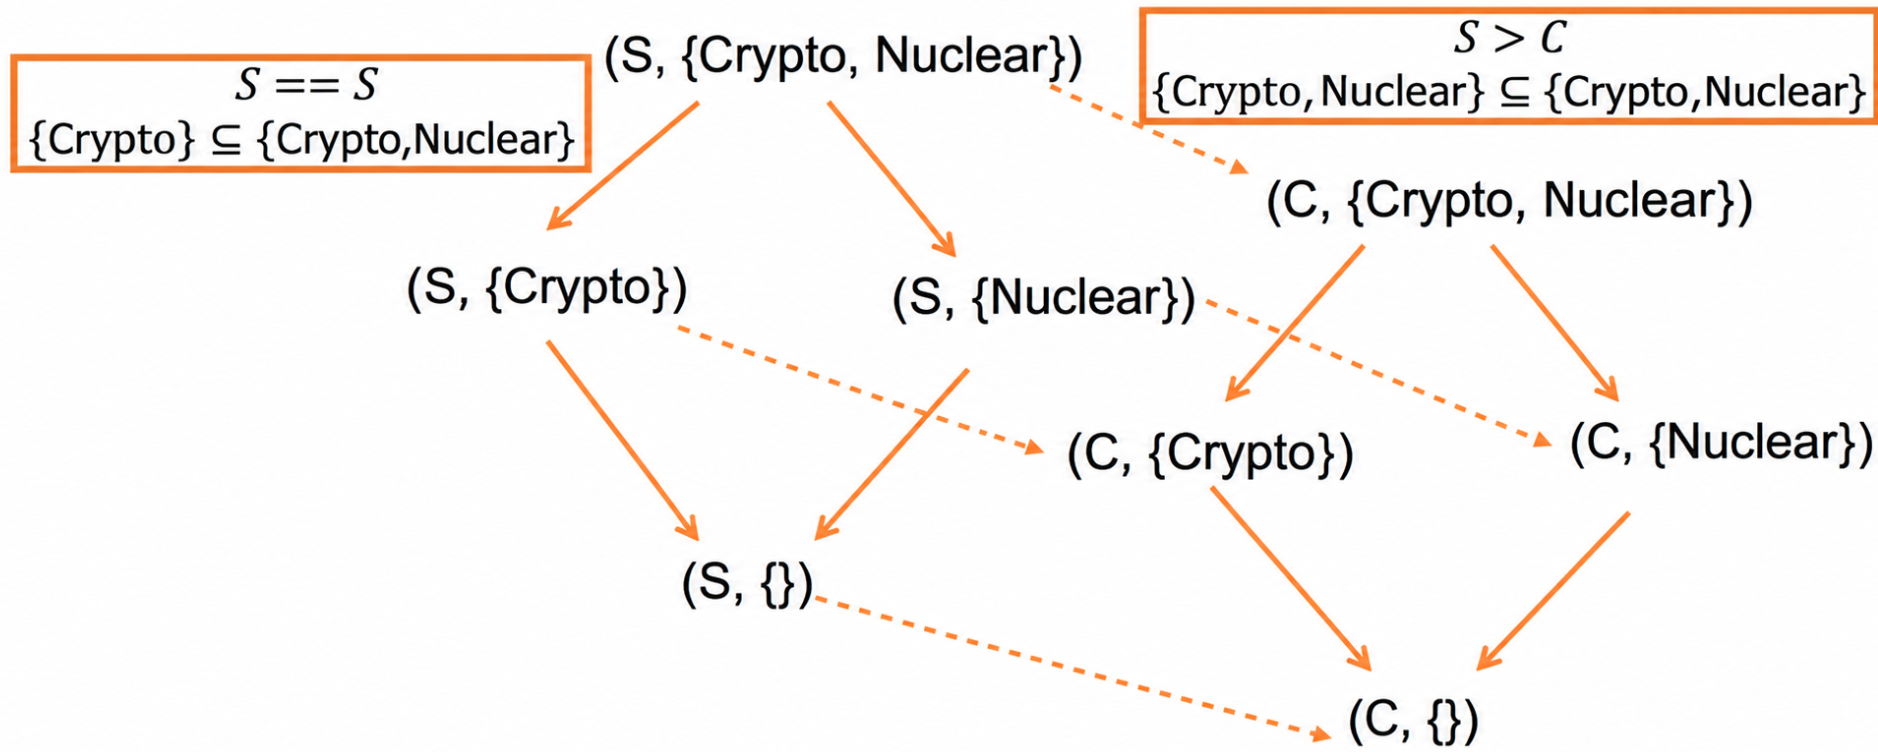
\includegraphics[width=0.8\linewidth]{images/img_20261010_173149.png}
\end{center}

With labels $C < S$ and categories Crypto, Nuclear we obtain $2 \times 2^2 = 8$ security levels, which can be drawn as a lattice (an arrow from $x$ to $y$ means $x \succeq y$: arrows point \emph{down}, from the dominating level to the dominated one; solid arrows keep the label and drop a category, dashed arrows keep the categories and lower the label):

\paragraph{Three key properties.}
\begin{enumerate}
    \item[(a)] \textbf{Dominance is transitive}: if $x \succeq y$ and $y \succeq z$ then $x \succeq z$ (it is also reflexive and antisymmetric).
    \item[(b)] There are \textbf{top and bottom elements}.
    \item[(c)] It is \textbf{only a partial order}: some pairs are \emph{incomparable}. For instance, neither $(S, \{\text{Crypto}\}) \succeq (S, \{\text{Nuclear}\})$ nor the converse holds; similarly $(S, \{\}) $ and $(C, \{\text{Crypto}\})$ are incomparable.
\end{enumerate}

\begin{remark}
Incomparability is important for exercises: if neither level dominates the other, then \emph{no} flow is allowed in either direction (neither read nor append/write), because every BLP rule requires a dominance.
\end{remark}

\subsection{Security levels of subjects: clearance}

BLP also calls it ``classification'', but for subjects we speak of \textbf{clearance}:
\begin{itemize}
    \item \textbf{Clearance} $\text{level}(s_i)$: the \textbf{maximum} security level the subject has been assigned.
    \item \textbf{Current security level} $\text{current-level}(s_i)$: subjects can \textbf{operate at lower security levels} than their clearance.
\end{itemize}
\[
\boxed{\text{level}(s_i) \succeq \text{current-level}(s_i)}
\]

\begin{remark}[Lowering the current level: what is allowed and what is not]
BLP reasons about \textbf{processes (sessions)} and what they have read, not about what a human remembers.
\begin{itemize}
    \item \textbf{Allowed}: a Top Secret general opens a \emph{new session} at current level Unclassified. In that session he can only read Unclassified objects, so the process writing the memo has \emph{never touched} Top Secret data: even a Trojan running in it has nothing secret to leak.
    \item \textbf{Forbidden}: a session that has \emph{already read} a Top Secret object lowers its level and then writes into an Unclassified object. The process holds Top Secret data in memory, so this is exactly the Trojan leak. The *-property forbids it: observing $O_1$ (TS) and altering $O_2$ (U) requires $\text{level}(O_2) \succeq \text{level}(O_1)$, which does not hold. Relabelling the process does not remove the information already in it.
\end{itemize}
BLP \textbf{cannot} prevent the general from typing a secret \emph{from memory} in his Unclassified session: the model controls flows inside the system (processes, files), not people's heads. Cleared humans are \emph{trusted} principals; BLP mainly protects against \textbf{software} (Trojans, bugs) acting with the user's authority.

\textbf{Exam pitfall (Midterm 2024)}: ``the casting director lowers his level to Unclassified and writes the cast list into the cast member's file'' is wrong. If it is the same process that read the Confidential cast list, it is a write down (forbidden). If it is a new Unclassified session, it cannot read the cast list, and typing it from memory is not a covert channel but a leak by a trusted human, outside the model.
\end{remark}

\subsection{The simple security property (ss-property): No Read Up}

\begin{definition}[Simple security property]
If $(\text{subject}, \text{object}, \text{r})$ is a current access, then
\[
\text{level}(\text{subject}) \succeq \text{level}(\text{object}).
\]
\end{definition}

This is \textbf{No Read Up (NRU)}: a subject with clearance Secret can read Unclassified, Classified and Secret objects, but not Top Secret ones.

\begin{center}
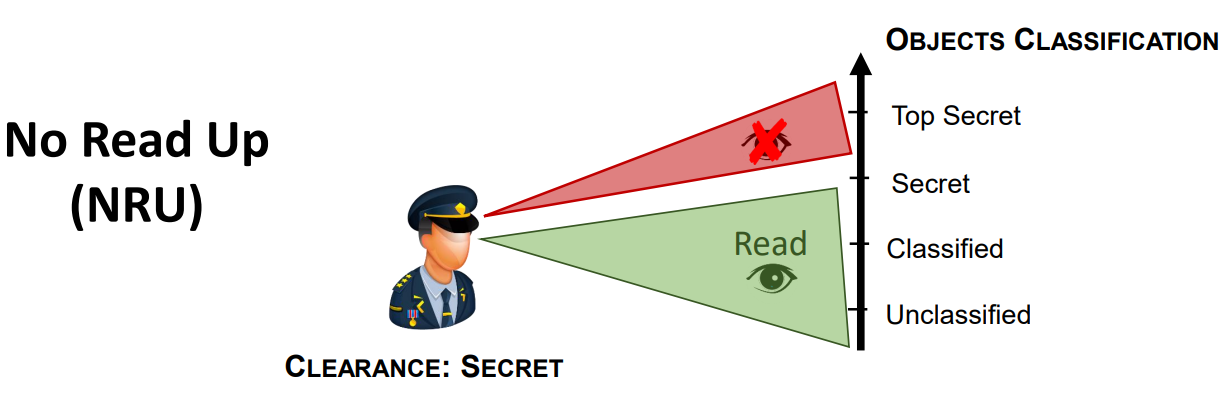
\includegraphics[width=0.707\linewidth]{images/img_20261010_181727.png}
\end{center}

\subsubsection{Why the ss-property is not sufficient}

\begin{center}
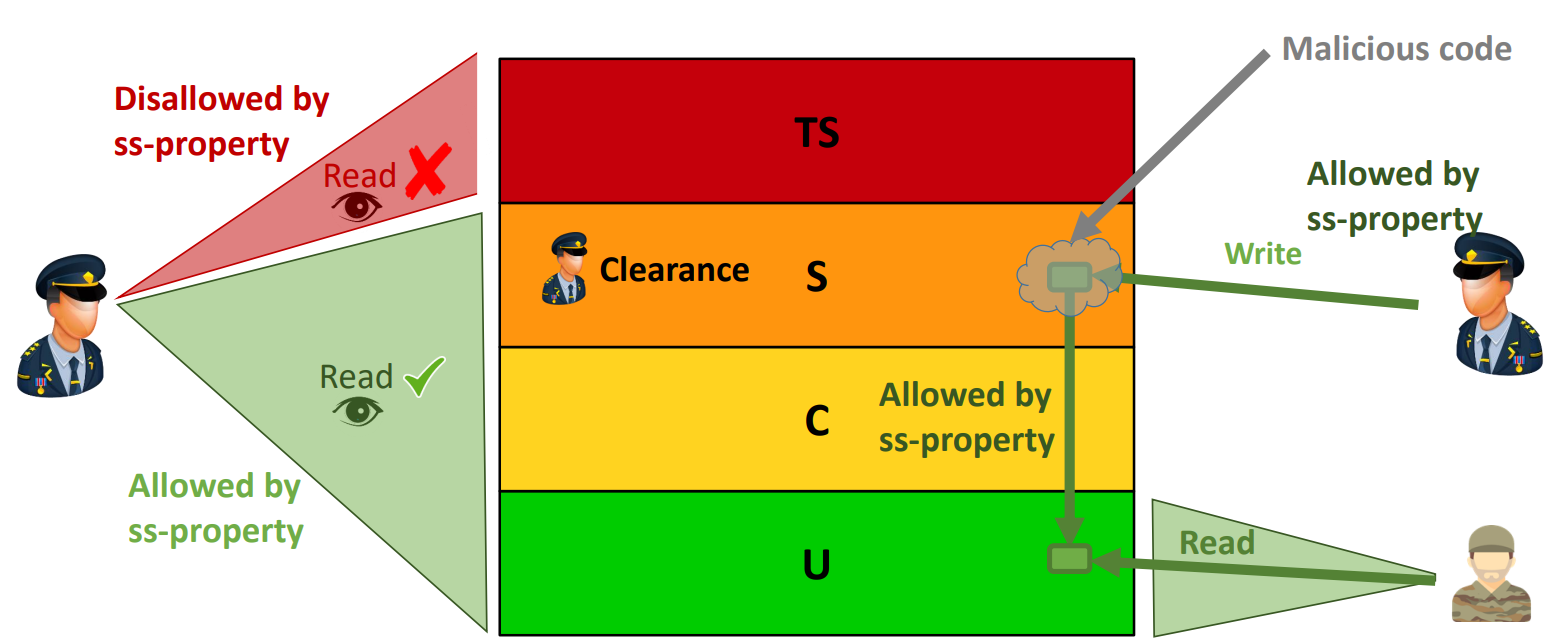
\includegraphics[width=0.707\linewidth]{images/img_20261010_181851.png}
\end{center}

The ss-property only constrains \emph{reading}. Consider a subject with clearance Secret who runs \textbf{malicious code} (a Trojan horse):
\begin{enumerate}
    \item the code reads a Secret object (allowed by the ss-property: Secret dominates Secret);
    \item the code writes its content into an Unclassified object (the ss-property says nothing about writing);
    \item any Unclassified subject reads the Unclassified object (allowed by the ss-property).
\end{enumerate}
Each individual step is allowed, but Secret information has \textbf{flowed down} to Unclassified. The user does not even need to be malicious: the program acts with the subject's authority. We need a rule on writing.

\subsection{The star property (*-property): No Write Down}

\begin{definition}[*-property]
If a subject has simultaneous ``observe'' access (r or w) to $O_1$ and ``alter'' access (a or w) to $O_2$, then
\[
\text{level}(O_2) \succeq \text{level}(O_1).
\]
\end{definition}

In practice, with respect to the current level of the subject, this gives \textbf{No Write Down (NWD)}: a subject may only \emph{alter} (append/write) objects whose level dominates its current level.

\begin{center}
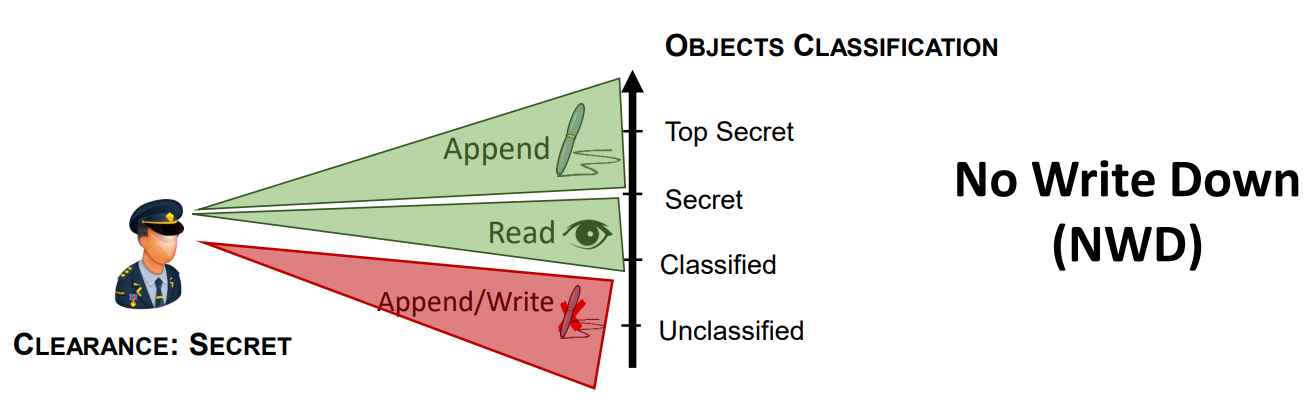
\includegraphics[width=0.707\linewidth]{images/img_20261010_182704.png}
\end{center}

\begin{remark}[Intuition]
\textbf{Read down, write up.} Information can only move from lower to higher levels. A Secret subject can \emph{append} to a Top Secret file (``blind write up'': it cannot read the result), which is harmless for confidentiality (but not for integrity, see BIBA!).
\end{remark}

\subsection{The discretionary property (ds-property)}

Information should only be accessed on a \textbf{need-to-know} basis: being cleared Secret does not mean you need \emph{every} Secret document. \textbf{MAC needs DAC} to implement least privilege \emph{inside} a security level. It is also important to protect integrity.

\begin{definition}[Discretionary security property]
If an access $(\text{subject}, \text{object}, \text{action})$ takes place, it \textbf{must be in the access control matrix}.
\end{definition}

So an access is granted only if \emph{both} the mandatory rules (ss, *) \emph{and} the discretionary matrix allow it.

\subsection{The Basic Security Theorem}

\begin{definition}[Basic Security Theorem]
If all state transitions are security preserving, and the initial state is secure, then every subsequent state is secure, regardless of the inputs.
\end{definition}

In other words, if for any individual access (1) the ss-property, (2) the *-property and (3) the ds-property are preserved, then security holds for any sequential composition of accesses. A system can be analysed in terms of \textbf{single-step state transitions}.

\begin{remark}
Is it surprising? \textbf{No}: it is essentially an induction over the sequence of states. Its value is methodological (check each transition locally), but it hides the real question: \emph{what are the transitions, and what does it mean to ``read'' something?}
\end{remark}

\begin{example}[One bit leaks through a transition]
Assume $\text{level}(s_1) = \text{TS}$ and $\text{level}(s_2) = \text{C}$.
\begin{enumerate}
    \item $s_2$ creates $o_2$, so $\text{level}(o_2) = \text{C}$.
    \item $s_1$ reads $o_2$ (allowed: read down) and then, depending on a Top Secret bit, either
    \begin{itemize}
        \item changes the object's level: $\text{level}(o_2) = \text{TS}$, or
        \item leaves it untouched: $\text{level}(o_2) = \text{C}$.
    \end{itemize}
    \item $s_2$ attempts to access $o_2$ at level C: \textbf{success or failure leaks 1 bit} of Top Secret information!
\end{enumerate}
Every transition looked ``secure'', yet information flowed down. The model does not capture the \emph{observable side effects} of transitions (here the success/failure of an access). This is a \textbf{covert channel}. (Such attacks motivate the idea that labels should not change while in use, often called \emph{tranquility}.)
\end{example}

\subsection{Covert channels}

\begin{definition}[Covert channel]
Any channel that allows \textbf{information flows contrary to the security policy}.
\end{definition}

The information is hidden inside actions or messages that the policy \emph{allows}. Two families:
\begin{itemize}
    \item \textbf{Storage channels}: the sender modifies a shared stored value that the receiver can observe. E.g.\ shared counters, ID fields, file metadata (names, sizes, existence of a file, lock state), \dots
    \item \textbf{Timing channels}: the sender modulates the timing of something the receiver can measure. E.g.\ use of the CPU, load to memory (cache), queuing time, \dots
\end{itemize}

\begin{remark}[Link with the principles]
The more resources are shared, the harder it is to eliminate covert channels. This is exactly \textbf{Principle 7: least common mechanism}: every shared mechanism (CPU, cache, file system, disk) is a potential communication path between levels.
\end{remark}

\paragraph{Mitigation.}
\begin{itemize}
    \item \textbf{Isolation}: make communication with the low level impossible (no shared resources).
    \item \textbf{Add noise} to the communication (e.g.\ random delays), which reduces the bandwidth.
\end{itemize}
Limits of mitigation:
\begin{itemize}
    \item It is hard to achieve less than \textbf{1 bit/s}.
    \item That is \textbf{OK for documents} (leaking a whole report takes a long time), but \textbf{NOT OK for cryptographic keys} (a 128-bit key leaks in about two minutes).
    \item Hence the DoD policy: \textbf{cryptographic keys must always be stored on dedicated hardware}.
\end{itemize}

\begin{remark}[Exam hints on covert channels (Midterm 2024)]
When asked to \emph{describe a covert channel}:
\begin{itemize}
    \item The channel must use \textbf{only actions the MAC allows} (read down, append up, shared resources). A channel that requires writing down (e.g.\ the high subject writing into an Unclassified file) \textbf{violates NWD} and is not a covert channel, it is simply forbidden.
    \item An \textbf{external} channel (phone, coffee shop, messaging app) with the message in the clear is \textbf{not} a covert channel: the information is not hidden inside an allowed action. (It is outside the system the MAC controls.)
    \item \textbf{Declassification is not a covert channel}: it is run by the policy (not the user), and it removes the sensitive content.
    \item \textbf{Encryption is not a covert channel}: an encrypted message written down is still a write down.
\end{itemize}
\end{remark}

\subsection{Declassification}

\begin{center}
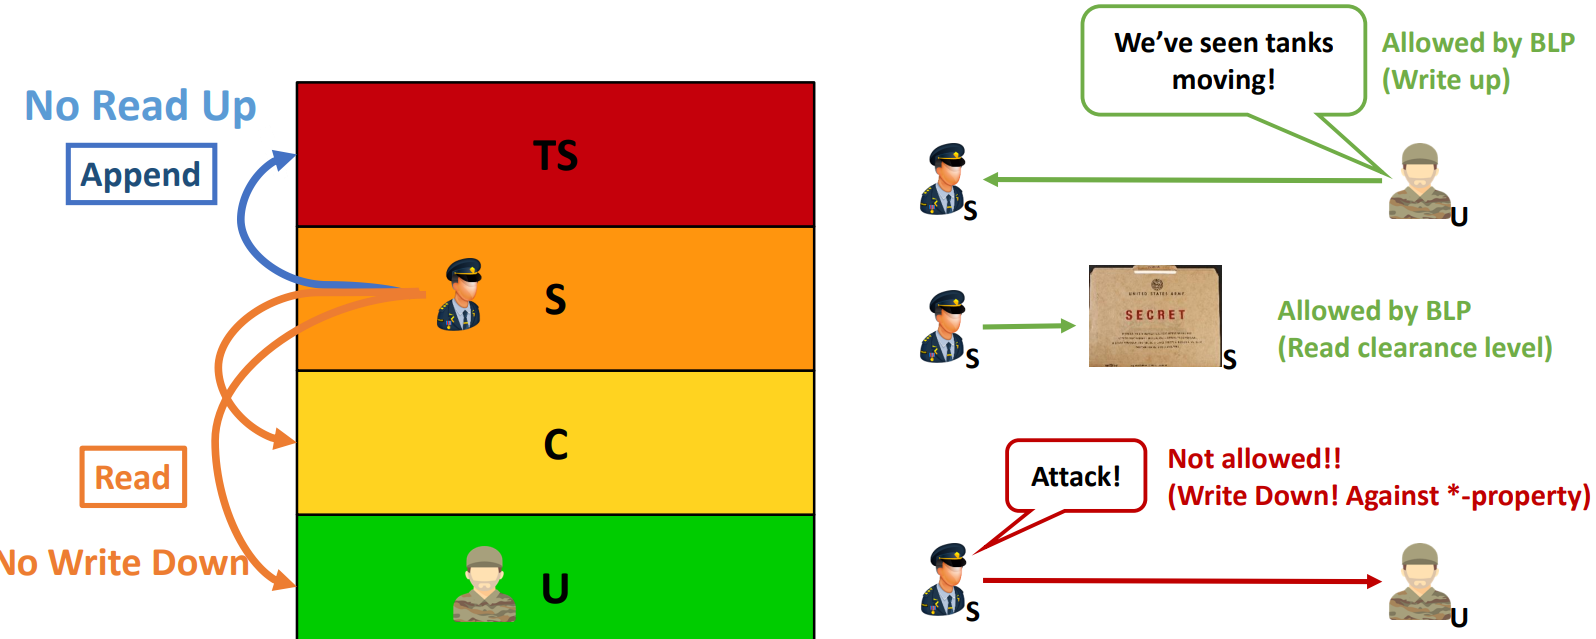
\includegraphics[width=0.8\linewidth]{images/img_20261010_184239.png}
\end{center}

\begin{example}[Tanks]
An Unclassified observer sees tanks moving and \emph{appends} ``We've seen tanks moving!'' to a Secret report (write up: allowed by BLP). The Secret commander reads it (read at his clearance level: allowed). He now wants to send ``Attack!'' to Unclassified soldiers: \textbf{this is a write down, not allowed by the *-property}. Yet the system is useless if orders can never reach the soldiers.
\end{example}

\begin{definition}[Declassification]
\textbf{Removing a classification label} (or lowering it) from an object.
\end{definition}

\begin{itemize}
    \item It is \textbf{very typical and necessary}: information must eventually flow down (orders, public reports, archives).
    \item It happens \textbf{under the control of the security policy}, not at the discretion of a user.
    \item It \textbf{cannot be made inherently safe}: it is a \textbf{manual process}, with rules about archives and historical records.
    \item It is \textbf{hard to rule out covert channels}: how do you know the object does not contain secrets (hidden in wording, whitespace, metadata, \dots)?
\end{itemize}

\subsubsection{Difficulty of declassification in practice}
\begin{itemize}
    \item \textbf{Microsoft Word revision history} retains deleted text.
    \item \textbf{PDF redaction} by overlaying graphical elements (usually black rectangles): \textbf{the text is still in the file}, and can be copied out.
    \item \textbf{Mosaicing and blurring} are ineffective for redacting text (Hill, Zhou, Saul, Shacham, PETS 2016): the hidden text can be recovered.
\end{itemize}
Always assume a \textbf{strategic adversary} who will look for every trace left.

\subsection{Limitations of BLP}

\begin{itemize}
    \item \textbf{Confidentiality-oriented}: it does not consider integrity or availability (a low subject may append garbage to a Top Secret file).
    \item \textbf{State-based, single-transition model}: too low-level and not expressive.
    \item The \textbf{three security properties are not sufficient} to ensure confidentiality (covert channels, as in the 1-bit example).
    \item \textbf{Changes} in clearance and classification can create covert channels\dots
    \item \dots but a \textbf{static system without changes is impractical} (hence the need for declassification).
\end{itemize}

\section{Integrity models}

\subsection{Why integrity?}

BLP focuses on confidentiality, which is relevant for military and government environments. What about \textbf{commercial services}? Banking, stock and sales inventory, stock exchange, land registry, student grades database, electronic contracts, payments, \dots

\begin{itemize}
    \item Preventing \textbf{fraud} is about protecting \textbf{integrity}: the adversary has not influenced the result.
    \item Confidentiality is either secondary or unnecessary.
\end{itemize}

\textbf{Integrity is key for computer security in general!}
\begin{itemize}
    \item The \textbf{TCB has to have high integrity} (if the reference monitor can be modified, no policy holds).
    \item \textbf{Public key cryptography requires high integrity for confidentiality}: if an adversary can replace Bob's public key with her own, encrypting ``to Bob'' gives the message to the adversary.
\end{itemize}

\subsection{The BIBA model}

Subjects and objects have \textbf{integrity levels}, from lowest integrity to high integrity. Two operations: \textbf{read} (observe) and \textbf{write} (modify). Two strict rules:

\begin{definition}[BIBA strict integrity rules]
\begin{itemize}
    \item \textbf{Simple integrity property (No Read Down)}: a subject may read an object only if $\text{level}(\text{object}) \succeq \text{level}(\text{subject})$. This \textbf{protects higher integrity principals from being corrupted by lower integrity data}.
    \item \textbf{*-integrity property (No Write Up)}: a subject may write an object only if $\text{level}(\text{subject}) \succeq \text{level}(\text{object})$. This \textbf{prevents lower integrity principals from corrupting high integrity data}.
\end{itemize}
\end{definition}

\begin{center}
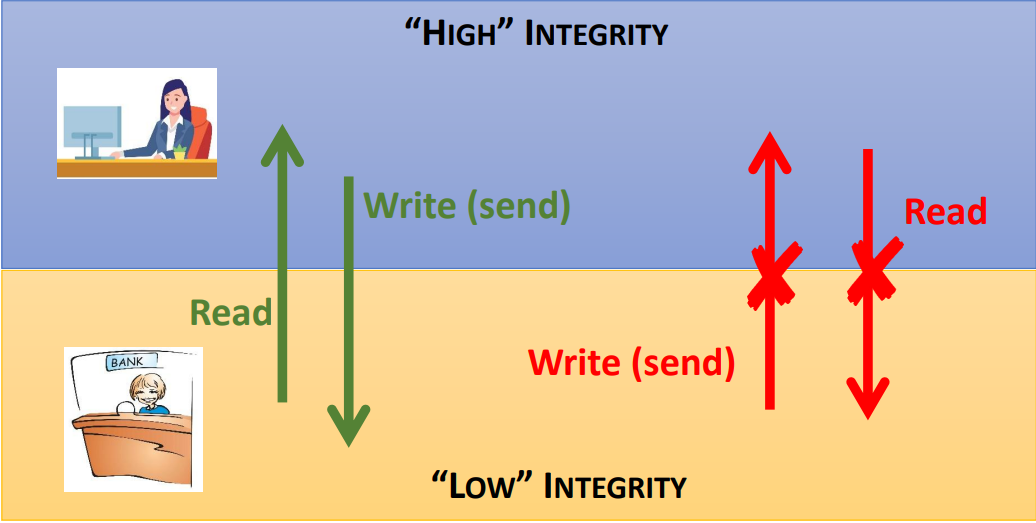
\includegraphics[width=0.6\linewidth]{images/img_20261010_191053.png}
\end{center}

BIBA is the \textbf{dual of BLP}: \textbf{read up, write down}. Information can only flow from high integrity to low integrity.

\begin{example}
\begin{itemize}
    \item \textbf{In the bank}: the director (high) can establish a rule and every employee (low) reads it (read up). Employees cannot rewrite the rules (no write up).
    \item \textbf{In the computer}: a web application open in the browser (low integrity, it processes untrusted network input) should not write to the file system (high integrity), at most to \texttt{/tmp}.
\end{itemize}
\end{example}

\begin{table}[h]
\centering
\begin{tabular}{@{}lll@{}}
\toprule
 & \textbf{BLP (confidentiality)} & \textbf{BIBA (integrity)} \\
\midrule
Read & No Read \textbf{Up} (read down) & No Read \textbf{Down} (read up) \\
Write & No Write \textbf{Down} (write up) & No Write \textbf{Up} (write down) \\
Information flows & upwards only & downwards only \\
Protects against & leaking secrets to low levels & corruption of high levels by low data \\
\bottomrule
\end{tabular}
\caption{BLP and BIBA are duals.}
\end{table}

\begin{remark}
Using BLP and BIBA together with the \emph{same} levels would forbid everything but same-level access. In practice they use different, independent labels.
\end{remark}

\subsection{BIBA variant 1: low-water-mark for subjects}

The strict rules are very rigid. A first relaxation:
\begin{itemize}
    \item Subjects \textbf{start processes at their highest integrity level}.
    \item When accessing (reading) an object, the subject's current level is \textbf{lowered to the lowest of the two}: $\text{current-level}(s) \gets \min(\text{current-level}(s), \text{level}(o))$.
\end{itemize}
So reading down is \emph{allowed}, but it ``contaminates'' the subject: once it has read low data, it can no longer write high objects.

\begin{center}
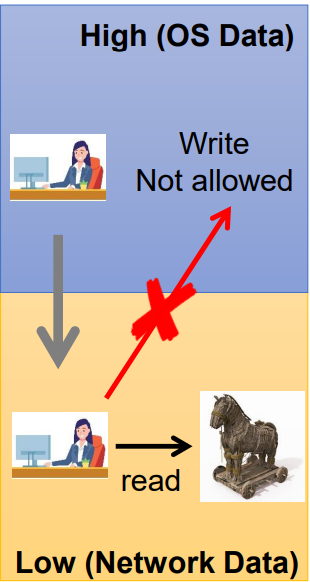
\includegraphics[width=0.2\linewidth]{images/img_20261010_191224.png}
\end{center}

\begin{itemize}
    \item It is a \textbf{temporary downgrade for the session}.
    \item Example: \textbf{mitigate the impact of a network Trojan}: a process that read network data (low) can no longer write OS data (high).
    \item Problem: it is \textbf{hard to avoid label creep}: subjects keep reading lower data, and after a while everything runs at the lowest level.
\end{itemize}

\subsection{BIBA variant 2: low-water-mark for objects}

\begin{itemize}
    \item Once an object has been written to by a subject, it \textbf{assumes the lowest level of the object and the subject}.
    \item Example: a high-integrity database written to by a process with access to the network (low integrity) is labelled ``low'' integrity.
\end{itemize}

\begin{center}
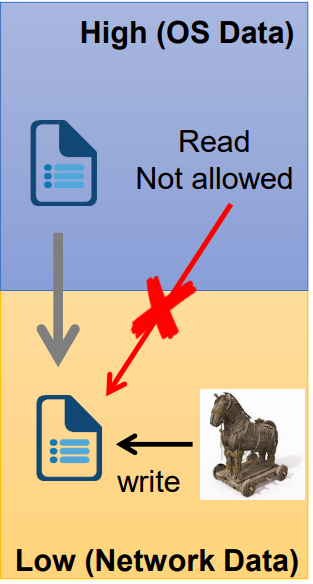
\includegraphics[width=0.2\linewidth]{images/img_20261010_191757.png}
\end{center}

\textbf{What is the effect?} Writing up is no longer prevented, the object is simply relabelled. This is \textbf{dangerous}: it only allows \textbf{detection} of integrity violations (after the fact), not prevention. Mitigation: \textbf{replicate objects} (keep a high-integrity copy) and \textbf{sanitize or erase} the contaminated ones.

\subsection{BIBA additional action: invoke}

Subjects can also \emph{invoke} (call) other subjects:
\begin{itemize}
    \item \textbf{Simple invocation}: only allow subjects to invoke subjects \textbf{with a label they dominate} (invoke lower or equal).
    \begin{itemize}
        \item[+] Protects high integrity data from misuse by low integrity principals (a low subject cannot drive a high subject).
        \item[$-$] What level is the output? (the result comes from a lower-integrity subject)
    \end{itemize}
    \item \textbf{Controlled invocation}: only allow subjects to invoke subjects \textbf{that dominate them} (invoke higher, e.g.\ through a well-defined interface such as a system call).
    \begin{itemize}
        \item[+] Prevents corruption of high integrity data: the high subject does the modification itself.
        \item[$-$] Hard to detect polluting information passed in by the low invoker (this is exactly the sanitization problem below).
    \end{itemize}
\end{itemize}

\subsection{Sanitization}

\begin{definition}[Sanitization]
The process of taking objects with ``\textbf{low}'' integrity and ``\textbf{lifting them}'' to ``\textbf{high}'' integrity.
\end{definition}

It is the integrity counterpart of declassification. ``Sanitization'' problems are \textbf{the root cause of large classes of real-world security vulnerabilities}: malformed ``low'' (user) input influences ``high'' (service) data and code.

\begin{example}
\begin{itemize}
    \item \textbf{Web security}: the web server (high) accepts input from the web client (low), passes it to an SQL interpreter $\to$ \textbf{SQL injection} vulnerability.
    \item \textbf{OS security}: a UNIX \textbf{suid} program (high) accepts input from a user (low) into a short buffer $\to$ \textbf{buffer overflow}.
\end{itemize}
\end{example}

\subsubsection{Fundamental principle of sanitization}

\textbf{Positively verify} that ``low'' objects are within a \textbf{valid set} before elevating their integrity to ``high''.
\begin{itemize}
    \item \textbf{Whitelist}: check that all properties of good objects hold.
    \item \textbf{Do not blacklist}: do not just check for bad objects or properties.
\end{itemize}
This is \textbf{Principle 2: fail-safe defaults}, ``base access decisions on permission rather than exclusion'' (Saltzer \& Schroeder, 1975).

The universe of good things is small and well-defined; the set of bad things is large and undefined. Asking ``is it in the universe of good things? accept'' is sound; asking ``is it in the set of bad things? reject'' always misses something (and covert channels are difficult to catch anyway).

\subsection{Principles to support integrity}

Three principles to guide design choices:
\begin{itemize}
    \item \textbf{Separation of duties}: require \textbf{multiple principals} to perform an operation. It is harder for an adversary to tamper with the system, as they have to corrupt two principals.
    \item \textbf{Rotation of duties}: allow a principal only a \textbf{limited time} in any particular role, and limit other actions while in this role. It is harder for an adversarial insider to tamper with the system (no time to set up a long-running fraud, and the successor may notice it).
    \item \textbf{Secure logging}: a \textbf{tamper-evident log} to recover from integrity failures. \textbf{Consistency of the log across multiple entities} is key. It is harder to make an integrity breach durable.
\end{itemize}

\begin{remark}[Integrity bootstraps other properties]
To \emph{bootstrap} means to build one property on top of another: \textbf{high integrity can be used to obtain high confidentiality or high availability}, and losing integrity can make you lose them too.
\begin{itemize}
    \item \textbf{Integrity $\Rightarrow$ confidentiality (PKI).} Alice encrypts a message for Bob with Bob's public key. If an adversary can \emph{replace} Bob's key in the directory with her own, Alice in fact encrypts for the adversary, who decrypts it, reads it, and re-encrypts it with Bob's real key so that nobody notices. The encryption is perfect, yet confidentiality is lost because the \emph{integrity of the key} was not guaranteed. A PKI (certificates signed by an authority) guarantees that ``this key belongs to Bob''; confidentiality then follows.
    \item \textbf{Integrity $\Rightarrow$ availability (replication).} To keep a service available, data is replicated on several servers: if one fails, another takes over. But a \emph{corrupted} replica may serve wrong data, or spread the corruption to the others during synchronization. If the integrity of each replica can be \emph{verified} (hashes, signatures), the bad copy is detected and a good one is used instead. Replication only gives availability if we know which replicas are sound.
    \item \textbf{Conversely}, a loss of integrity leads to \textbf{low confidentiality} or \textbf{low availability}
\end{itemize}
This is why integrity is central in computer security: the \textbf{TCB itself must have high integrity}, otherwise no other property holds.
\end{remark}\section{The Chinese Wall model}

D.\ F.\ C.\ Brewer and M.\ J.\ Nash, \emph{The Chinese Wall Security Policy}, IEEE S\&P 1989.

\subsection{Motivation}

Inspiration: UK rules about handling \textbf{conflicts of interest} in the financial sector.
\begin{itemize}
    \item A separation must exist \textbf{at all times}, even within the same firm, between people engaging in activities that conflict with each other (e.g.\ a consultant advising two competing companies).
    \item Cost of failure: large fines and reputation.
\end{itemize}

\subsection{Entities and basic concepts}

\begin{enumerate}
    \item All objects are associated with a \textbf{label denoting their origin}: ``Pepsi Ltd.'', ``Coca-Cola Co.'', ``Microsoft Audit'', ``Microsoft Investments''.
    \item The originators define \textbf{conflict sets} of labels: $\{\text{Pepsi Ltd.}, \text{Coca-Cola Co.}\}$, \\$\{\text{Microsoft Audit}, \text{Microsoft Investments}\}$.
    \item Subjects are associated with a \textbf{history of their accesses} to objects, and in particular of their labels.
\end{enumerate}

\begin{remark}
Unlike BLP and BIBA, the Chinese Wall is \textbf{dynamic}: what a subject may access depends on what it has accessed \emph{before}. Initially, a subject may access anything; each access builds the wall.
\end{remark}

\subsection{Access rule}

\begin{definition}[Chinese Wall access rule]
A subject can access an object (for either read or write) if the access \textbf{does not allow an information flow between items with labels in the same conflict set}.
\end{definition}

\begin{center}
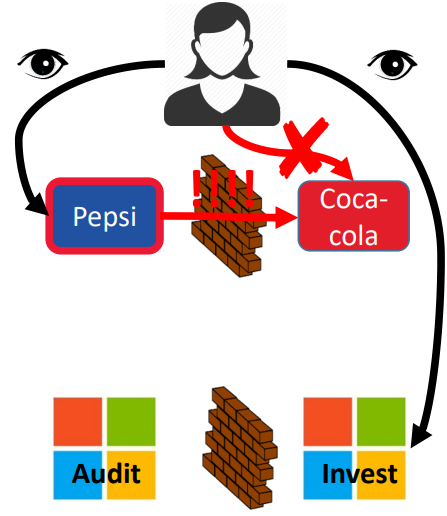
\includegraphics[width=0.25\linewidth]{images/img_20261010_193420.png}
\end{center}

\begin{example}[Direct flow]
Alice starts her first day at work.
\begin{enumerate}
    \item She accesses files of ``Pepsi Ltd.'': OK (empty history).
    \item She accesses files of ``Microsoft Investments'': OK (different conflict set).
    \item She tries to access files of ``Coca-Cola Co.'': \textbf{access denied}!
\end{enumerate}
Why? She has already accessed files of ``Pepsi Ltd.'', so an information flow between Pepsi and Coca-Cola, in the same conflict set, might happen (she could work again with Pepsi). Similarly, she can no longer access ``Microsoft Audit''.
\end{example}

\subsection{Indirect flows}

Direct flows within a conflict set are easy to detect. What about indirect ones?

\begin{center}
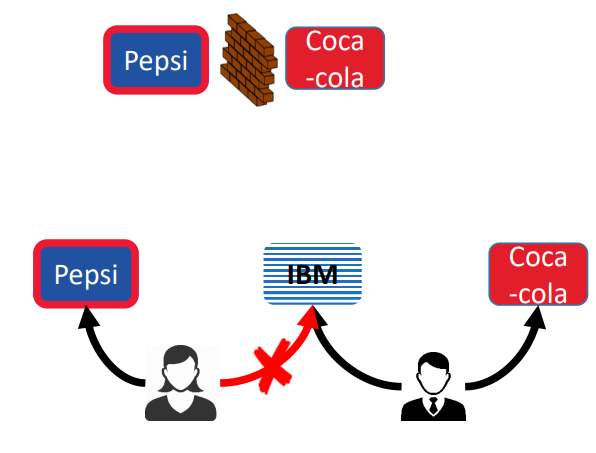
\includegraphics[width=0.4\linewidth]{images/img_20261010_193716.png}
\end{center}

\begin{example}[Indirect flow]
Alice and Bob start together.
\begin{enumerate}
    \item Alice is assigned to ``Pepsi Ltd.'': OK.
    \item Bob is assigned to ``Coca-Cola Co.'' and ``IBM Co.'': OK (IBM is not in conflict with Coca-Cola).
    \item Alice tries to access files of ``IBM Co.'': \textbf{access denied}!
\end{enumerate}
Why? If she writes into IBM files with her knowledge of Pepsi, Bob can read them, and the information may flow to Coca-Cola. Information flows \textbf{transitively} through objects shared by different subjects, so the model must track flows, not only direct accesses.
\end{example}

\paragraph{Sanitization is necessary for business.} If every shared object blocks everyone, nobody can work. Some items are therefore ``\textbf{un-labelled}'' as long as the information \textbf{cannot lead to any conflict of interest}, e.g.\ extracting some ``general market information''. Sanitized objects can be accessed by anybody without building a wall.

\subsection{Multilateral security}

BLP and BIBA are \emph{multilevel}: flows are vertical between ordered levels. The Chinese Wall is an example of \textbf{multilateral security}: the constraints are \emph{between} parties at the same level (lateral), whose interests and security properties conflict with each other. It protects both confidentiality (Pepsi's secrets do not reach Coca-Cola) and integrity (advice to Coca-Cola is not influenced by Pepsi's interests).

\section{Summary}

\begin{itemize}
    \item \textbf{MAC}: a central policy decides, and it must hold even against subjects trying to subvert it. \textbf{Security models} are design patterns for MAC policies; the devil is in the details (subjects, objects, mechanisms).
    \item \textbf{Security level} $=(\text{classification}, \{\text{categories}\})$. $(l_1, c_1) \succeq (l_2, c_2)$ iff $l_1 \geq l_2$ and $c_2 \subseteq c_1$. Dominance is a transitive \textbf{partial order} forming a lattice with top and bottom; some levels are incomparable.
    \item Subjects have a \textbf{clearance} (maximum level) and a \textbf{current level} it dominates.
    \item \textbf{BLP} (confidentiality): \textbf{ss-property} (No Read Up), \textbf{*-property} (No Write Down; observe $O_1$ and alter $O_2$ requires $\text{level}(O_2) \succeq \text{level}(O_1)$), \textbf{ds-property} (access must be in the matrix: need-to-know, MAC needs DAC). Read $\Rightarrow$ down, append $\Rightarrow$ up, write $\Rightarrow$ same level.
    \item \textbf{Basic Security Theorem}: secure initial state $+$ secure transitions $\Rightarrow$ every state is secure. Not sufficient in practice: \textbf{covert channels} (storage, timing) leak information through allowed actions; more sharing means more channels (least common mechanism). Mitigation: isolation, noise; $< 1$ bit/s is hard, so keys go on dedicated hardware.
    \item \textbf{Declassification}: necessary, under the control of the policy, manual, never inherently safe (Word history, PDF black boxes, blurring).
    \item BLP limitations: only confidentiality, too low-level, properties insufficient, changes create covert channels, static systems impractical.
    \item \textbf{BIBA} (integrity, the dual of BLP): \textbf{No Read Down}, \textbf{No Write Up}. Variants: low-water-mark for subjects (label creep), for objects (only detection; replicate and sanitize). Invocation: simple vs.\ controlled.
    \item \textbf{Sanitization}: lifting low-integrity objects to high integrity; root cause of SQL injection, buffer overflows, XSS. Use \textbf{whitelists, not blacklists} (fail-safe defaults).
    \item Integrity principles: \textbf{separation of duties}, \textbf{rotation of duties}, \textbf{secure logging}. Integrity can bootstrap confidentiality (PKI) and availability (replication).
    \item \textbf{Chinese Wall}: origin labels, conflict sets, access history; deny any access allowing a flow between labels of the same conflict set, including \textbf{indirect flows}. Sanitized ``general'' information is un-labelled. An example of \textbf{multilateral security}.
\end{itemize}
